%\documentclass[letter]{article}
\documentclass[letter,12pt]{article}
\usepackage[letterpaper,right=1.25in,left=1.25in,top=1in,bottom=1in]{geometry}
\usepackage{setspace}

\usepackage{hyperref}
\usepackage{url}
\usepackage[pdftex]{graphicx}
\usepackage[longnamesfirst, sort]{natbib}\bibpunct[]{(}{)}{,}{a}{}{;}
\usepackage{arydshln}
\usepackage{amsmath}

%\usepackage{rotating}
%\usepackage{pdflscape}

\newcommand{\mc}{\multicolumn}

\graphicspath{{../graphs/}}

\begin{document}

\title{Transparency, Automated Redistricting,  and Partisan Strategic Interaction: \\ 
       The Case of Mexico\thanks{Paper prepared for delivery at the Annual Meeting of the American Political Science Association, Washington, DC, August 2014. We thank the Federal Electoral Institute (IFE) and the Federal Voter Registry (RFE). Special thanks to IFE's Cartography Department for sharing their experience with automated redistricting since 1996 and most of the data we analyze. We also acknowledge the support from the Asociaci\'on Mexicana de Cultura A.C.\ and CONACYT for this work.}}

\author{Alejandro Trelles {\small \url{lat44@pitt.edu}} \\
        Micah Altman {\small \url{escience@mit.edu}} \\
        Eric Magar {\small \url{emagar@itam.mx}} \\  
        Michael McDonald {\small \url{michael.mcdonald@ufl.edu}}
      }
\date{\today}
\maketitle


\begin{abstract}
%Abstract Version 1 
\noindent In the U.S.\ redistricting is deeply politicized and often synonymous with gerrymandering ---the manipulation of boundaries to promote the goals of parties, incumbents, and racial groups. In contrast, Mexico's federal redistricting has been implemented nationwide since 1996 through automated algorithms devised by the electoral management body (EMB) in consultation with political parties. In this setting, parties interact strategically and generate counterproposals to the algorithmically generated plans in a closed-door process that is not revealed outside the bureaucracy. The way that redistricting has played out so far in Mexico raises a number of questions: Were the plans produced algorithmically, in fact, optimal with respect to the selected criteria? How did partisan counterproposals differ from the bureaucratic solution? What influence did parties have on the final plan? Can automated and partisan interactive  models  generate relatively fair and unbiased plans?  We address these questions by analyzing a novel dataset that has never been available outside of the EMB and that comprises the entire set of plans proposed by political parties during the 2013 redistricting process.  Our analysis offers a unique insight into the internal workings of a purportedly autonomous EMB and the institutional challenges derived from the lack of transparency in drawing electoral maps.

\end{abstract}

%Comment[Alejandro]: Micah will suggest a new line/structure in order for the paper to have consistency around a general argument and Alejandro will adapt the paper that outline. 

 %Comment[Alejandro]: As we have discussed, and from comments we have received from external reader, the main limitation of the paper is the lack of clarity in terms of laying down a theory and some hypotheses. It reads more like a descriptive policy piece with recommendations than a traditional poli sci paper. 
  
% Comment [Eric]: Possible argument for the presentation: 1) Expert committees can remove partisan bias from redistricting; 2) Mexico's process allows parties to respond. Offers leverage to infer party preferences and degree of influence; and 3) Analysis of party bias and responsiveness informs this, directly. 

% Comment [Alejandro]: That is a possibility (arguing that "Expert committees can remove partisan bias from redistricting"), but so far the paper is framed in a way where we cast doubt regarding how autonomous EMBs, despite being independent, still have spaces to improve, serious transparency challenges and might still produce biased plans... I am not sure if these two points (Eric's suggestion and how the paper is framed so far) are mutually exclusive, but it  might be harder to make a strong case if we decide to move in this direction. I highlighted Eric's second point ("2) Mexico's process allows parties to respond. Offers leverage to infer party preferences and degree of influence") in the "Assesment subsection." Perhaps we can leave the farming as it is and underline the positive aspects in part of the text and in the conclusions. 

\onehalfspacing

Electoral institutions in democratic settings usually serve the purpose of translating the peoples' will, expressed by their votes, into the selection of representatives that enact policies. In redistricting --- the periodic drawing of electoral boundaries, ostensibly to achieve seemingly apolitical goals such as balancing districts' populations --- the causal chain can be reversed. The drawing of new electoral boundaries may allocate voters to districts in ways that affect the number of legislative seats parties are expected to win, the careers of incumbents, and representation for racial and other interest groups. With so much at stake, scholars have found the redistricting process can distort representation, through an eponymous strategy known as gerrymandering \citep{mayhew1974vanishingMg,cox.katz.2002,erikson1972malapportionment,engstrom2006redisttrictApsr}. 

Some state governments in the US have sought to remove the opportunity for politicians to engage in gerrymandering by shifting redistricting authority from state legislatures to independent boundary commissions; although some commissions' rules and membership continue to produce highly politicized outcomes, while others less so \citep{mcdonald.CommVsLegisRedistrict2004,trelles.mtz.polygob2012}. Mexicans similarly decided to overcome this challenge by delegating redistricting authority to the Federal Electoral Institute (IFE, now INE), an independent election management board created in the early 1990s. Mexico has innovated beyond the U.S.\ by employing self-tailored automated algorithms to find redistricting plans deemed optimal on \emph{a priori} criteria, and for political parties to react by offering counter-proposals \citep{trelles.mtz.polygob2012}. Here, we examine the extent to which technocrats have supplanted politicians \citep{lujambio.vives.2008} by analyzing a novel dataset describing partisan interaction within IFE in the 2013 redistricting process.

Despite that electoral officials may claim to be politically neutral, scholars find the rules by which they operate may not constrain political manipulation \citep{lijphart.1990,rossiter.etal.1997,estevez.magar.rosas.2008}. Furthermore, criteria may embody subtle second order biases that produce a predictable political outcome \citep{parker.1990}. Rather than removing political bias, redistricting by commission may perpetuate it in a different guise. In particular, IFE conducts redistricting behind closed doors, without public scrutiny, much less public participation \citep{trelles.mtz.tesisItam.2007,trelles.datosabiertos.2015}.\footnote{The lack of information in previous redistricting rounds, even within the IFE, generated non-functional districts. In 1997 and 2006, for instance, electoral commissioners received complains --- from several local IFE commissions and party representatives in states like Sonora and Chihuahua --- arguing that they where not allowed to participate in the redistricting process and that several districts, despite being "optimal," where splitting communities or had major geographical accidents making them dysfunctional for organizational and campaign purposes \citep{trelles.mtz.tesisItam.2007}.} The media and public are provided insufficient information to assess if the final plan embodies political mischief --- for example, how the plan produced by automation methods differs from the final plan --- before the new plan is formally adopted by IFE's Council General and takes effect \citep{trelles.datosabiertos.2015}.

% Comment [Alejandro]: I added the following reference (trelles.datosabiertos.2015) to the redMex.bib file on GitHub (Eric, could you please verify if the bibliography file is working? I was not sure which of the two files on Github is the correct one (magar.bib file and a redMex.bib, I could only open the latter and bibliography is not being recognized): "citep{trelles.datosabiertos.2015" as follows: Trelles, Alejandro, Micah Altman, Eric Magar and Michael McDonald. 2015. Datos abiertos, representaci�n pol�tica y redistritaci�n en M�xico.  Pol�tica y Gobierno. Under Review. Available at SSRN.}

In 2015, as in 1997 and 2006, IFE employed an algorithmic redistricting process based upon criteria agreed amongst IFE's electoral commissioners before plans were drawn. IFE used the 2005 algorithm (a simulated annealing combinatorial optimization heuristic) with the same four input parameters (population balance, compactness, municipal integrity and traveling time), but with a slightly re-weighted overall scoring function to optimize \citep{trelles.mtz.tesisItam.2007,acuerdoife2013}. \footnote{In 1997 the algorithm was known within IFE as the "heuristic model" (it was an algorithm that aggregated \emph{secciones} from West to East and from North to South in each state balancing population and trying not to split municipal administrative divisions (traveling time, compactness and minority districts were not in the picture yet); in 2006, IFE used a simulated annealing algorithm for the first time (a heuristic with a cost function that aggregated \emph{secciones} departing from a randomly chosen seed that evaluated results under a high-low "temperature" dynamic. It was in this round (2006) where four differently weighted criteria  were introduced for the first time; In 2015, IFE decided to use again the simulated annealing algorithm and the same 4 criteria weighted slightly different. Bee hive optimization was considered by the Technical Committee, but was discarded because the cost function was not improved significantly.} As in 2006, the base geography was modified so that the algorithm could not partition: a) municipalities that had the sufficient population to form a district, and b) minority municipalities with at least 40\% of indigenous population \footnote{25 minority districts were created in 2015 and 28 in 2006}. 

The last redistricting process towards the 2015 election offers an opportunity to assess the robustness of Mexico's redistricting process. For the first time, IFE created a web-based map sharing tool, which allows us to analyze all redistricting plans formally introduced throughout the process. A large number of plans were produced, more than in any previous redistricting, and IFE'��s Technical Redistricting Committee enabled strategic interaction between entities by allowing them to observe counter-proposals formulated by other parties through the platform. \footnote{The idea of partisan interaction was introduced in the International Redistricting Seminar celebrated at IFE in Mexico City in November 2012. IFE had allowed parties to formulate observations in 1996 and 2005, but no interaction platform existed so that parties could observe what others were proposing. The authors of this paper introduced the idea during the presentation of the Public Mapping Project Mexico (www.publicmapping.org), an open source web based platform that allows citizens and parties to analyze redistricting scenarios, observe what other users are proposing, and formulate counterproposals in order to optimize the criteria established by the legal framework and allow the authority in charge of redistricting to automatically rank and evaluate counterproposals.} 

In the end, despite consensus within party representatives at IFE to endorse the final plan (they actively participated in the process), unexpected partisan resistance in the three major national party headquarters (PAN, PRI and PRD) stalled adoption of IFE's final plan and ushered in a set of reforms to the Mexican electoral system in early 2014. The way that redistricting has played out so far in Mexico and the last set of electoral reforms ---specially the reintroduction of legislative reelection starting in 2018 and the centralization of local congressional redistricting in a single national electoral management body (INE)--- raise a number of questions: Are the adopted redistricting criteria politically neutral? Were the plans produced algorithmically, in fact, optimal with respect to the selected criteria? How did partisan counterproposals differ from the bureaucratic solution? What influence did parties have on the final plan? Can automated and partisan interactive  models  generate relatively fair and unbiased plans?

In this work we answer these questions and assess Mexico's redistricting process in search of partisan effects on representation by inspecting data that has never been available outside of the Mexican government. It comprises the machine generated plans and two rounds of strategic counter-proposals made by political parties. In the following lines we discuss how differences across parties affected their participation in the redistricting process;  what do their choices tell us about their incentives; how was a machine-based solution affected by human interaction; and the  extent to which the process can be validated by the public given the existing levels of transparency. 

\section{Rules of the Game and Challenges for Transparency}

Mexico adopted a mixed-member electoral system for the lower house of Congress in 1978. In the first election, three hundred single-member districts were drawn to elect three-fourths of the chamber by plurality rule. \footnote{In order to simplify our argument, we decided to leave out of this analysis boundary delimitation for proportional representation seats. PR boundary delimitation has taken place  in 1979, 1982, 1985, 1997, and 2006 and we discuss these changes and its effects on representation in the following article: Eric Magar, Alejandro Trelles, Micah Altman, and Michael McDonald. 2015. The Effects of PR Boundary Delimitation on Representation: The Case of Mexico. Working Paper. University of pittsburgh.} That proportion fell to three-fifths since 1985, but the number of single-member districts (300) has not changed. Districts were not redrawn until 1996, coinciding with the first free and fair national election in 1997 \citep{lujambio.vives.2008,trelles.mtz.tesisItam.2007}. A third redistricting occurred in 2005, and a fourth process  took place in 2013, but was aborted. In the following lines we refer to district maps by the first year they were in use, not by the actual year they were drawn.\footnote{Despite maps were actually drawn in 1978, 1996, 2005, and 2013, we use years to name the different maps, sticking to the convention of using not the date when boundaries were actually redrawn and accepted, but that of the first election the map was (or would have been) used. Thus, there is a ``1979 map'' actually drawn in 1978, a ``1997 map'' drawn in 1996, a ``2006 map'' drawn in 2004--05, and a ``2015 map'' drawn in 2013, but never used.}

The method adopted has relied on machine-assisted mapping since 1997. Details have changed, but the broad lines have not \citep{trelles.mtz.tesisItam.2007}. Although a purportedly autonomous EMB has been in charge of supervising and administrating the boundary delimitation process, the lack of transparency and information availability do not allow the  public scrutiny to ensure that the configuration of electoral maps will remain unbiased \citep{trelles.datosabiertos.2015}. In the following lines we describe the three major stages of the redistricting process and what we believe are the main challenges for the electoral authority in Mexico: a) the apportionment of seats to states; b) the design of an optimization algorithm; and c) the strategic assessment of computer-generated district blueprints by a technocrats with active, but limited involvement of political parties.

\textbf{a) Apportionment}. This is the fist stage of the process and it basically consists in the redistribution of a fixed number of seats (300) among the 32 states.\footnote{The Federal District, where Mexico City resides, is not recognized as a state in the constitution, but is treated as one for the purpose of apportionment and redistricting.} Restrictions, reminiscent of the U.S., apply: no state may have fewer than two seats; the sole redistributive criterion above that minimum is state population; and no district may cross state boundaries.  

In contrast with the U.S., there has been no public debate about alternative methods of apportionment that could be used \citep{szpiro.numbersRule.2010,balinski.rodriguez.1996}. The Hamilton method of largest remainders is used \citep[][:10]{balinskiYoung2001FairRep}. The quota $Q$ (or price of a seat) is the nation's population divided by 300, the number of seats. A first allocation is made by dividing each state's population in the last general census by $Q$, rounded down. States with populations $<2Q$ nonetheless get two seats. Unallocated seats, if any, are awarded to states with largest fractional remainders. 

The first problem derived from this stage is that malapportionment is introduced. In previous rounds (1996 and 2006), for instance, persistent malapportionment was explained, in part, by the allocation of two seats to small states \citep{magar.etal.bias.2015}. Relative over-representation of tiny Southern Baja and Colima was substantial, but only until recently. Population growth has made both worth their congressional seats. Yet relative over-representation remains substantial in migrant-worker-exporter Zacatecas up to 2003, and in the Federal District of late. Both states have lost population fast relative to the rest, and the system's design makes rapid demographic shifts slip away from grip. 

A second problem, as discussed in \citep{magar.etal.bias.2015}, distortions have been usually introduced in this stage when the census counts that are used for redistricting are allowed to become out of date \citep[also see][]{snyder.samuelsMalapp2004}. The constitution mandates the use of the census for redistricting, but sets no obligation to redistrict as soon as it becomes available. As a consequence, drawing a new map for 2015 with data from the year 2010 injects a fair amount of creeping malapportionment into the new plan right at its inception \citep{magar.etal.bias.2015}. With this in mind, it is puzzling that the redistributive nature of apportionment has not pushed for the adoption of alternative methods. The seventeen states that were under-represented in 2006 jointly controlled a majority (162) of single-member districts; fourteen of them have always been in this situation. 

% Comment [Alejandro]: I added the reference of the Bias paper  to the redMex.bib file on GitHub (Eric, could you please verify if the bibliography file is working? I was not sure which of the two files on Github is the correct one (magar.bib file and a redMex.bib, I could only open the latter and bibliography is not being recognized): "\citep{magar.etal.bias.2015" as follows:  Magar, Eric, Alejandro Trelles, Micah Altman, and Michael McDonald. 2015. The effects of malapportionment, turnout and gerrymandering in Mexico's mixed-member system. Working Paper. University of Pittsburgh.}

\textbf{b) Optimization}. The second stage brakes in two phases. In the first phase municipalities --- also known as \emph{municipios} (the lowest elected offices, similar to counties in the U.S.)---  that have at least 40\% of indigenous population or that, by their population size, qualify to conform a district (within the respective +/- 10\% or  +/- 15\% deviation allowed) are identified and cannot be split during the optimization process. Both of these criteria, indigenous population and municipal integrity, are embedded in the redisctricting agreements approved by IFE's General Council in 2004 and 2013 (\citep{acuerdo.ife.2004,acuerdo.ife.2013}). 

% Comment [Alejandro]: I added the following references (acuerdo.ife.2004,acuerdo.ife.2013) to the redMex.bib file on GitHub (Eric, could you please verify if the bibliography file is working? I was not sure which of the two files on Github is the correct one (magar.bib file and a redMex.bib, I could only open the latter and bibliography is not being recognized).

In the second phase, a new map is drawn from the base geography by adopting of a set of desiderata. The optimization algorithm runs three separate times departing from different randomly selected seeds. It makes marginal changes to boundaries, repeatedly reassigning geographical blocks --- \emph{secciones electorales} --- between districts, and systematically checking tradeoffs between criteria in a formal cost function. Cost-minimizing district maps for each state are thus generated and the map with the lowest cost is selected as the first scenario (``scenario 1'') \citep{trelles.mtz.tesisItam.2007}. \footnote{The building blocks are more than 66 thousand \emph{secciones electorales} into which the Mexican territory is subdivided. \emph{Secciones} are analogous to U.S.\ census tracts, but somewhat bigger. Median \emph{secci\'on} population in the 2010 census was 1,280 persons, with a maximum at 79,232.} Other restrictions also apply: contiguity is a must and no district can have enclaves.  

The simulated annealing optimization heuristic described in the last paragraph, and used to generate the 2015 map, had a slightly re-weighted overall scoring function that included four criteria (and relative weights): population balance (.4), municipal boundary preservation (.3), traveling times inside the district (.2), and district compactness (.1).\footnote{In the previous round (for the 2006 map) the four criteria were the same but they were wighted slightly different (relative weights): population balance (.4), district compactness (.3), municipal boundary preservation (.2), and traveling times within the district's municipal headquarters (.1).} IFE would tolerate population deviations of up to +/- 15\% across districts, and deviations above that threshold with proper justification \citep{acuerdo.ife.2013}. The EMB began working on this process on August, 2012 and almost one year later, the technical committee presented the 2015 map proposal (``scenario 1'') on July 17, 2013. 

The first problem with the optimization stage has to do with the arbitrariness in how criteria are selected, operationalized, and weighted in a cost function. The legal framework mentions that parameters such as population balance and minority districts with indigenous population should be considered, but it does not specify the sequence, methods, components or rules of the game to be followed during the redistricting process. The spirit behind using a differentiated weighing system for the four components (population balance, municipal boundary preservation, traveling times inside the district, and district compactness) was to prioritize the relevance each component. However, the components were never normalized making it imposible for the algorithm to weight them properly and for the technical committee to compare the cost between components. 

In 2006, for instance, the technical committee decided that if the value associated to the cost function for two scenarios was the same, population growth at the district level would be considered in order to determine which map should prevail. \footnote{This criterion --- population growth --- had no legal basis and it was used in 2006 in Mexico City (DF) to determine that the municipality of Coyoac\'an should receive an additional district, instead of Iztapalapa (\citep{ife.memorias.2005}).}  Furthermore, while population was defined in IFE's redistricting agreements (\citep{acuerdo.ife.2004,acuerdo.ife.2013}) as the only first order and most important criterion it gave it a weight of only 40\%, compared to the 60\% aggregated value it gave to the other three components. \footnote{As described in \citep{trelles.mtz.tesisItam.2007}, an alternative weighing system for the same four components could have been used (e.g. population balance (.7), district compactness (.2), municipal boundary preservation (.06), and traveling times within the district's municipal headquarters (.04).}  It is in these details where we believe there is an important gap and an opportunity for the EMB to increase significantly the levels of public awareness, eliminate areas of opacity, and improve the technical justification around the different stages of the process.

% Comment [Alejandro]: I added the following references (ife.memorias.2005) to the redMex.bib file on GitHub (Eric, could you please verify if the bibliography file is working? I was not sure which of the two files on Github is the correct one (magar.bib file and a redMex.bib, I could only open the latter and bibliography is not being recognized).

A second problem is the gradually changing criteria with no apparent technical or legal justification. As described above, in 1997 IFE used a "heuristic model" that aggregated \emph{secciones} from West to East and from North to South in each state balancing population and trying not to split municipal administrative divisions (\citep{trelles.mtz.tesisItam.2007}).\footnote{Traveling time, compactness and minority districts were not in the picture yet}; In 2006, IFE used a simulated annealing algorithm for the first time that had a cost function --- restricted by four differently weighted components --- that aggregated \emph{secciones} departing from a randomly chosen seed; In 2015, the same simulated annealing heuristic was used, but the priority of components changed (\citep{acuerdo.ife.2006,acuerdo.ife.2013}).\footnote{Population balance remained the most important component with a weight of (.4), but compactness went from being the second order component with a weight of (.3) to the last place (.1), municipal boundary preservation became the second most relevant component (.3), and traveling time shifted from being the less important component in 2006 to the third place in 2015 having a weight of (.2).} 

After the 2014 electoral reform, Mexico's EMB (now INE) acquired national administrative attributes and, among other things, became responsible for electoral administration in the 32 states, including the redistricting processes for local legislatures.\footnote{Before 2014, each state had its own autonomous EMB} In 2015, INE became in charge of redistricting five states (Aguascalientes, Baja California, Durango, Tamaulipas and Zacatecas); in 2016 they will renew the cartography in eight states (Chihuahua, Hidalgo, Oaxaca, Puebla, Quintana Roo, Sinaloa, Tlaxcala and Veracruz); and two more in 2017 (Coahuila and Nayarit). For redistricting at the local level, the EMB made two major changes: a) they decided to use a bee optimization search algorithm; and b) they decided that during the the first phase of the optimization process they would consider indigenous population, municipal boundary preservation and traveling time across municipal headquarters to identify municipalities that would not be split by the algorithm. For the second phase of the optimization, the EMB decided to use only two --- instead of four --- components (with the respective weights): a) population balance (1) and b) district compactness (.5).\citep{ine.modelo.2015} In the cost function, the former received twice as much of the weight compared to the latter to reflect the priority of the components. It is unclear what the optimization method, weighing system or components will be used if the EMB decided to renew the 300 federal electoral districts for the 2018 election. 

So far the EMB has not been able to justify these changes and, given the lack of transparency and public awareness surrounding the redistricting processes, we consider this ambiguity is one of the major challenges for the EMB. Although automated redistricting has been successfully applied by Mexico's EMB for almost two decades,\footnote{Compared to other countries that periodically update their constituency boundaries, Mexico's redistricting processes are usually not challenged in courts.}  the process is far from being transparent and its rigidity to allow different social actors --- civil society, interest groups, regional parties, media, NGOs, academics --- to engage, audit, understand and actively participate in these processes, represents an important risk for  redistricting to become a highly politicized process, especially when legislative reelection is reintroduced in 2018. 

% Comment [Alejandro]: I added the following references (ine.modelo.2015) to the redMex.bib file on GitHub (Eric, could you please verify if the bibliography file is working? I was not sure which of the two files on Github is the correct one (magar.bib file and a redMex.bib, I could only open the latter and bibliography is not being recognized).

A third problem derived from the optimization stage is the wide margins allowed for population deviation. Neither the constitution nor the electoral law specify that a population deviation should be allowed between districts. It was the EMB, through the agreements approved by its General Council, that approved a deviation of up to +/- 15\%.\footnote{In states where the district average population deviated less than 5\% from the national average, a deviation of up to +/- 15\% was allowed, whereas in states with deviations above 5\%, a margin of only +/- 10\% was permitted (\citep{acuerdo.ife.2004,trelles.mtz.tesisItam.2007})}. In 2006, for instance, districts in 23 of the 32 states where allowed to have a deviation of up to +/- 15\% while the rest was allowed only to have a deviation up to +/- 10\% (\citep{trelles.mtz.tesisItam.2007}). As with the population growth criterion, there is no legal basis --- or technical justification --- that determine why having districts where populations exactly at the bounds of the $\pm15$ spread --- which basically means that citizens at the bottom end would be worth one-third more in Congress than those at the top end --- is something desirable or reasonable, especially when the main objective of the process is to safeguard the "one man, one vote" principle. 

Unequally-sized districts has been a common practice in Mexico in spite of the automated application of clear quantitative redistricting criteria since 1997. In fact, Mexican parties in general, and IFE in particular, have been remarkably tolerant of this practice. As a consequence, this form of malapportionment is related, in some degree, to states' imbalanced apportionment in Congress, which perforce creates size differences across states' mean district sizes. But size inequality within states is also prevalent and substantial (\citep{magar.etal.bias.2015}). We recognize that small deviations around a state's mean district population are unavoidable, especially as a map ages. But what constitutes significant deviation depends on the political context. Courts in the U.S.\ have struck down new district maps bearing less than 1\% differences without proper justification \citep{tuckerApportionment.1985}. Redistricting authorities generally view a \emph{de minimus} population deviations of as little as one or zero persons between congressional districts as desirable to inoculate against litigation. In stark contrast, IFE has allowed deviations up to 15\% (since 1997) above or below mean state district size (\citep{lujambio.vives.2008,trelles.mtz.polygob2012}) and, surprisingly, no party has ever challenged this practice in Court. 

\textbf{c) Assessment}. The third stage begins once the first scenario has been formally presented by IFE's technical committee --- appointed by the Council General --- and distributed to political parties. It involves two rounds where technical experts comment on the maps and political parties observe and suggest modifications to the maps.\footnote{This stage took approximately four months. It began in July 2013 and concluded in October 2013.} Amendments are proposed to the first scenario, and those that are adopted by the technical committee are then used as a starting point for another round of partisan observations to produce a second scenario. Parties are invited again to propose a second round of amendments and, once they have been analyzed and discussed by the technical committee, a final plan is presented to the Council General to be formally approved. 

In both, 2006 and 2015 rounds, the technical committee decided that the assessment of plans would: a) consider the value associated to the cost function. That is, plans with a lower cost were preferred to alternatives with higher values;\footnote{As discussed below, this rule has not always been followed} and b) do not consider counterproposals --- even if they had a lower cost --- that compromised any of the decisions that were made during the first phase of the optimization process (i.e. splitting municipalities with a high concentration of indigenous population or municipalities that had the population to form a district and that were previously identified as such by the committee).  

In the 2015 round, IFE invited two sets of institutional actors to participate in the process: the seven national parties represented in the National Surveillance Commission (NSC) and the same seven parties represented in each of the 32 state-based Local Surveillance Commissions (LSC).\footnote{Involving the LSC allowed the EMB to be more aware of local issues and interests across the 32 states.} Compared to the 2006 process, the inclusion of the LSCs allowed the active participation of local bureaucrats and party representatives at the state level. The development of a web based mapping tool was extremely useful for EMBs bureaucrats in Mexico City's headquarters to receive party counterproposals across the country in real time.

The major innovation made in the 2015 round, was that IFE created a web based platform for parties to participate, interact and observe in real time the counterproposals made by other parties and electoral bureaucrats (CNV and LSCs). This offered the EMB a leverage to infer party preferences and allowed parties to have a degree of influence in the plans. The automated generated plans minimized the cost function, but the different rounds of counterproposals show that humans can defeat the machine (\citep{altman.mcdonald2011bard}). This stage also gave party representatives at the state level, for the first time, the possibility to make explicit demands to incorporate community and local interests in the new plans.

As it occurs in most administrative processes, mistakes took place during the assessment process. In both 2006 and 2015 redistricting rounds,  miscommunication between the EMB and parties was evident. Most parties ---especially at the local level --- submitted counterproposals with the idea that plans that did not improve the cost function, but that had a social or communitarian justification, were going to be considered by the committee. In 2006, for instance, the private secretary of the governor of Oaxaca (a state ruled back then by the PRI), through its party representative at the CNV, sent a petition to consider an alternative map to the committee asking not to consider the cost function. In the state of Michoac\'an, the governor sent a similar petition, signed by all political parties, asking the technical committee to consider a plan that was way above the cost function, but that was more "reasonable" in terms of representing community interests in the state's capital. In the 2015 round, political parties presented a significant number of counterproposals with a higher cost than the one obtained for the first and second scenarios arguing in favor of community interests. In both cases, the technical committee decided to consider only those counterproposals that were equal or decreased the value of the cost function.  

At the same time, some parties formulated counterproposals that were bellow the first and second scenarios, but that were rejected by the committee. After interviewing former members of the technical committee and to electoral officials, what explains these cases is that parties had access to a software that allowed them to split all municipalities, even those with a high concentration of indigenous population or that had the population to form a district, and that were previously identified by the committee in the first phase of optimization. There have been several cases in the 2006 and 2015 redistricting rounds where the golden rule of using the value associated with the cost function as a reference to decide which plan is "better" has been broken. This has happened in the state of Jalisco in 2006 (against PAN) and in Baja California Sur (against MC), Durango (against PRD), Morelos (against PRD), Quer\'etaro (against PRD) and Tabasco (against PRI and PVEM) in 2015, and are precedents that affect the perception of different actors regarding the consistency, objectivity and transparency of the rules being applied by the EMB.  From our perspective, this is a major challenge that the EMB needs to solve in the subsequent redistricting rounds. 

Some lessons to be learned from the evolution of automated redistricting: a) The rules of the game ---for all three major stages of the process ---  need to be clear. If they change over time, there needs to be a legal and technical justification; b) Consistency. All rules and procedures should be applied in the same way across cases and over time to decrease the levels of uncertainty; c) Communication between electoral officials and political parties needs open and formal procedures should be available for all parties. All actors should be able to express their interests and understand how to communicate them formally. At the same time, the authority should be clear in how those interests will be processed; d) Transparency, information availability and public scrutiny are crucial to guarantee the impartiality of redistricting; e) New forms to receive and evaluate public input during the redistricting process need to be developed.  So far, the redistricting process in Mexico is restricted to electoral bureaucrats and political parties. However, both parties and the EMB could be benefitted by opening the process to the public. The recent electoral reform, for instance, allows independent candidates to compete for legislative offices. However, political parties are the only actors allowed to participate in the process. Other social voices and interest groups could be considered during the redistricting process if the proper channels are developed.\footnote{By experiences in other countries, we know that new mapping technologies and the use of web based platforms make public mapping both feasible and convenient.}   

\section{Partisan Strategic Interaction}

Political parties interact strategically with mapmakers, and other parties, and propose amendments to the computer-generated plans, but these amendments must improve the overall cost score to be considered for adoption. Table \ref{T:counterprops} summarizes the two rounds of amendments that took place in preparation for the 2015 map. The number of proposals increased significantly over previous redistricting, because IFE expanded participation to the its state offices, giving the parties two channels to deliver simultaneous counter-proposals. There were a total of 534 counterproposals made for the 2015 map (more than twice of the counterproposals made for the 1997 and 2006 maps). 236 counterproposals were made to the first scenario (157 from the LSC and 79 form the NSC) and 308 were made to the second scenario (139 by the LSC and 169 by NSC).

Parties actively challenged proposed districts, making 75 counter-proposals each on average. Although we expected that all 7 parties would behave as rational self-interest maximizers and strategically make competitive counter-proposals to the first scenario, the right-of-center PAN was, by far, the most successful. Nearly half of their 82 proposals were accepted, compared to about one-fifth for the other major parties (PRI and PRD).\footnote{After talking with party representatives at the CNV, and former members of the technical committee, it seems that this is partly because PAN was the most technically prepared party. On the other, other parties have followed an appointment system for their representatives at CNV and the LSCs based on party quotas and camaraderie, rather than professionalization.} Amendments originated in both national (7 parties at the National Surveillance Commission) and state level (same 7 parties represented at 32 Local Surveillance Commissions).\footnote{The full set of parties represented in each committee were PAN, PRI, PRD, PT, PVEM, MC and PNA.} Activity at the amendment stage was enhanced by the adoption of an internal web-based map-sharing tool, which standardized counter-proposals and enabled parties to observe each others' amendments --- improving information for strategic behavior. The final proposal for Council General approval was presented on October 15, 2013. In the midst of a major electoral reform that took place in December that year, the Council General, driven by the pressure of the three major parties (PAN, PRI and PRD), chose not to decide before the end of the year. The 2015 midterm election, it was soon after learned, would be held with significantly outdated districts (based on the 2000 census results). 

\begin{table}
\begin{center}
  \begin{tabular}{lrrr|rrr|r}
    Party & national & state  & total 1st & national& state  & total 2nd & Total \\ \hline
    PAN   & 17/22    & 2/20   & 19/42     & 17/24   & 4/16   & 21/40     & 40/82 \\
    PRI   & 0/0      & 2/28   & 2/28      & 8/30    & 6/26   & 14/56     & 16/84 \\
    PRD   & 3/27     & 2/21   & 5/48      & 5/29    & 5/18   & 10/47     & 15/95 \\
    PT    & 1/12     & 1/20   & 2/32      & 3/15    & 1/16   & 4/31      & 6/63 \\
    PVEM  & 0/0      & 1/20   & 1/20      & 7/28    & 3/17   & 10/45     & 11/65 \\
    MC    & 1/17     & 0/21   & 1/38      & 6/32    & 2/16   & 8/48      & 9/86 \\
    PNA   & 0/1      & 1/18   & 1/19      & 4/11    & 3/17   & 7/28      & 8/47 \\
    IFE   & 0/0      & 1/9    & 1/9       & 0/0     & 5/13   & 5/13      & 6/22 \\ \hline
    Total & 22/79    & 10/157 & 32/236    & 50/169  & 29/139 & 43/308    & 111/544 \\
  \end{tabular}
  \caption{Counter-proposals to the first and second scenarios at the National and Local Surveillance Committees. Denominator reports the number of counter-proposals made, numerator how many were adopted. Prepared by authors with information from the Federal Electoral Institute.}\label{T:counterprops}
\end{center}
\end{table}

We investigate how the 2015 redistricting process unfolded in Figure 1. For each of Mexico's thirty-two states we plot the overall score for each proposed redistricting plan (the value of the algorithm's cost function for the three scenarios are black points, numbered). The optimization objective is to produce a plan with the least cost, so plans with lower values are better than plans with higher values. The first scenario resulted from the optimization algorithm prior to party feedback, the second and third from party amendments. Colored points are party counteproposals to the second scenario, blue for the PAN, red for the PRI, yellow for the PRD, grey for the best offer by a minor party.\footnote{The same analysis for party reactions to the first proposal would reveal another interesting aspect of negotiation. A successful amendment in the first round sets the starting point for the optimization process towards the second round, and this might lend important proposal power. PAN was, by far, the most successful party in the first round.} Brown points represent two or more counter-proposals with equal scores, with one protruding petal for each plan. The cost function is expressed relative to the value of the second proposal. 

%\begin{landscape}
\begin{figure}
\begin{center}
    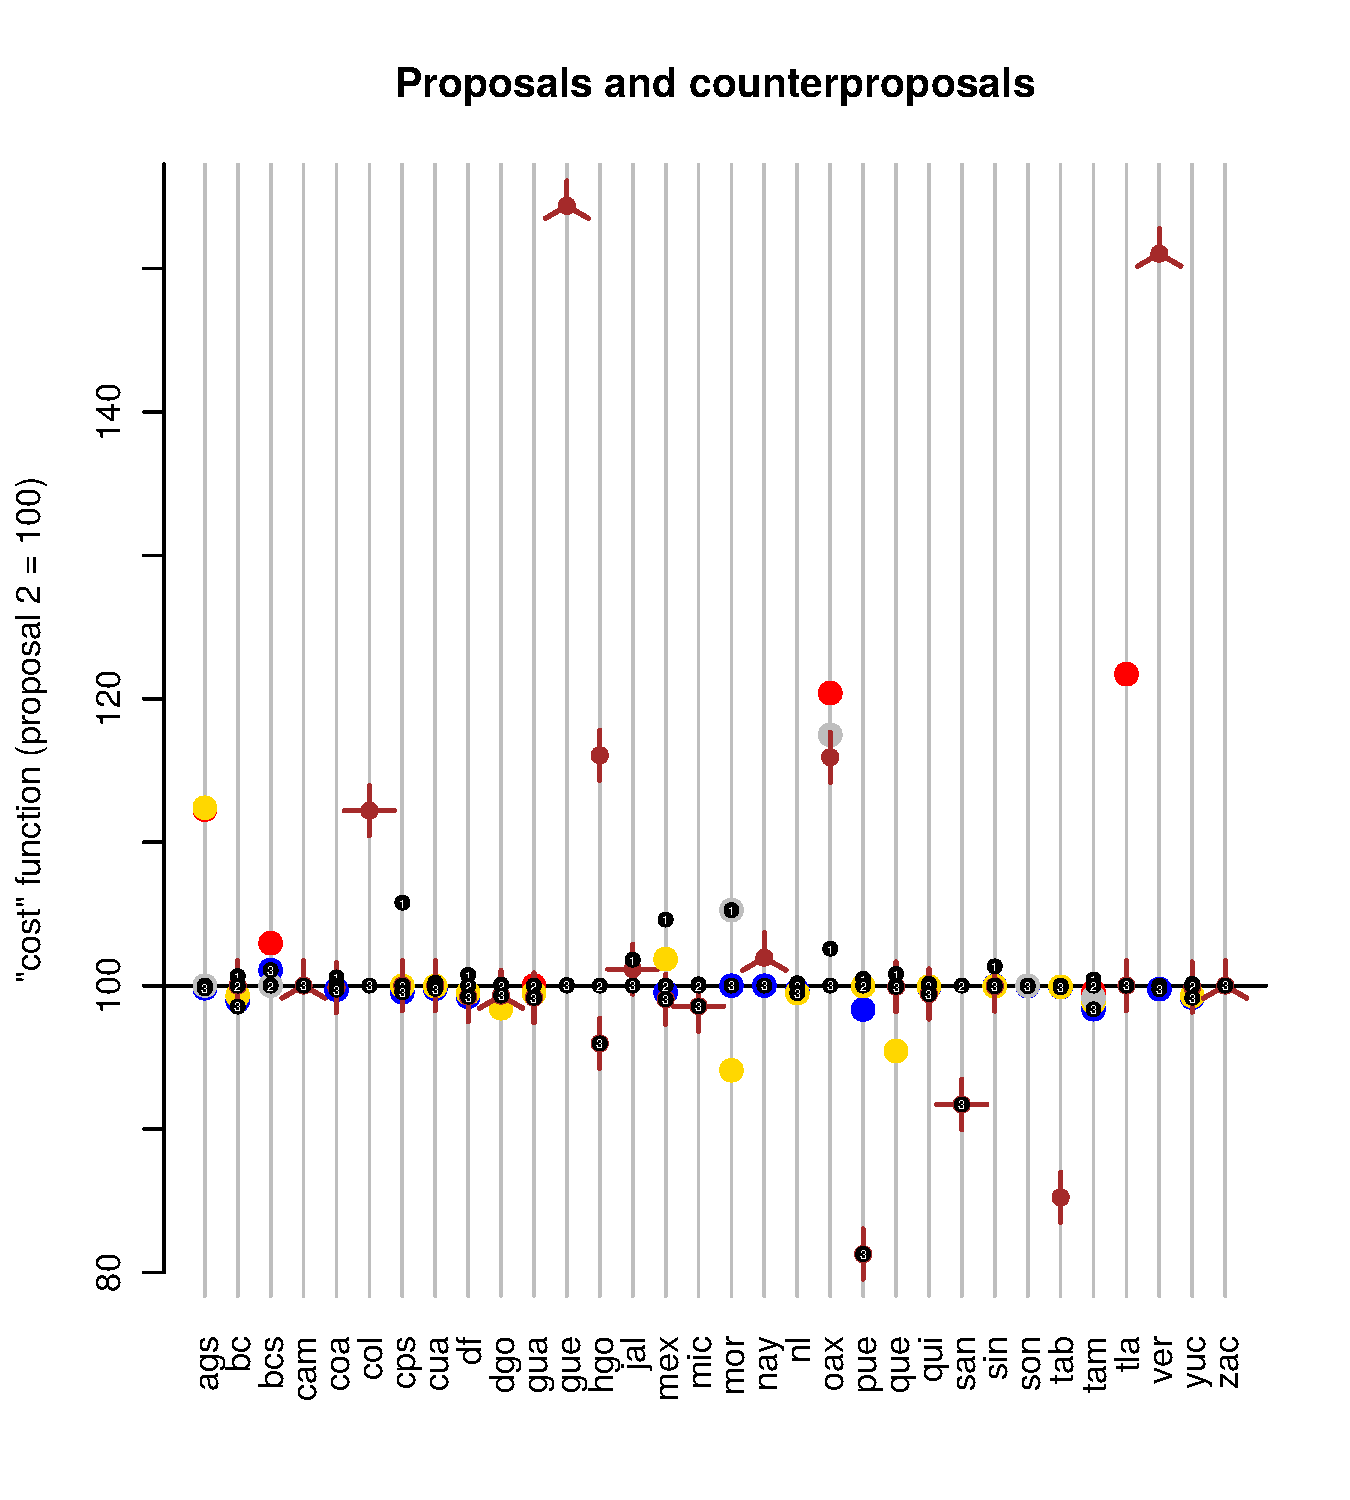
\includegraphics[width=\columnwidth]{propsAndCost.pdf} \\
  \caption{Map proposals towards 2015 by state. Black, numbered points indicate the value of the algorithm's cost function for the three map scenarios. The cost function is expressed relative to the value of the second proposal. Colored points are party counterproposals to the second proposal, blue for the PAN, red for the PRI, gold for the PRD, grey for the best offer by a minor party. Brown points report overlaps of two or more counter-proposals, one protruding petal for each overlap.}\label{F:propsAndCost}
\end{center}
\end{figure}
%\end{landscape}

In all but one state (Baja California Sur, BCS), the progression of scenarios is towards improving the cost function, as the third and final scenario has a lower score than either of the two prior scenarios.\footnote{In the case of BCS the algorithm first scenario had a cost function of 70.10687929, and PAN representative at the CNV made the counterproposal with the lowest value (70.09024166) during the first round of observations, which became the departing scenario for the second round of observations. In that second round, the PAN made a second counterproposal with an associated cost of 70.84932449. Despite another party, Movimiento Ciudadano (MC), had a preference for the scenario of 70.09024166, the technical committee decided to stay with the second proposal of the PAN.} We observe numerous instances where humans "beat" the machine, by offering counter-proposals that improve the first scenario's score. These plans demonstrate how redistricting is a complex integer optimization problem where optimization algorithms can become stuck in local optima \citep{altman.mcdonald2011bard}. Where the adopted amendments to the first scenario improve the score greatly --- as is the case in Hidalgo (Hgo), Puebla (Pue) and San Luis Potos\'i (San) --- the second round of counterproposals fails to further improve the previous round given that the margin to make changes becomes narrower. We cannot know for certain if these final plans are the global optimum since the algorithm departed from a randomly chosen seed and redistricting is such a challenging optimization problem.

There are three instances where the PRD offered a counter-proposal improving upon the first scenario and all other amendments, but the amendment was rejected: Durango (Dgo), Morelos (Mor), and Quere\'taro (Que). Two identical plans proposed in Tabasco (Tab) similarly are the objectively best plans, but are rejected. In these three instances, a second round of partisan observations fails to find better plans. This provides further evidence of how automated algorithms are challenged by the complexities of redistricting. More importantly, the existence of these better plans demonstrates that politics is present in the process, likely to the detriment of the PRD.   

% comment [Mike] We should say more about the politics behind these three rejected PRD plans. Also, was the PRD one of the two parties proposing plans for Tabasco?
% comment [Alejandro] We do not have the records on these cases, but I already emailed Miguel. Regardless of the answer, these decisions reveal a lack of consistency from the technical committee and it has been pointed out in the previous section. 

There are several proposals that have identical scores to the first scenario, and several instances where two proposals have identical scores. If two scenarios were tied, the technical committee would adopt the proposal that had lower cost values associated to the most relevant criteria --- population, followed by municipal boundary delimitation, traveling time and compactness at the end \citep{acuerdoife2013}. Further investigation may reveal subtle differences between these seemingly-similar plans, such as the assignment of two \emph{secciones} to different districts that has minimal changes on the overall score. We also observe numerous instances where parties propose plans that score worse than the first scenario. In many cases, as in 2005, parties decided --- even if the cost function of their counterproposal was higher than the departing scenario --- to present their plan and try to argue that their plan represented better specific communities or that responded better to geographical or socioeconomic characteristics not considered by the optimization algorithm.

In another key respect, all processes have remained opaque activities between electoral regulators and party representatives. New technology letting anyone interested, with little more than an Internet connection, see proposals, react, and improve them through crowd-sourcing or an open web based platform \citep{altman.mcdonald2011bard,trelles.datosabiertos.2015}, remains to be adopted. We observe evidence to suggest such transparency may not be welcome by all parties, as the PRD proposed objectively better plans that were never adopted.

\section{The 2006 Map and the 2015 Proposals}

A new map is a full description of district boundary changes. The common way to visualize a map is by drawing it. We look at maps differently, with focus not in the physical lines and line changes but in their political consequences. Putting the 2006 map and the 2015 final proposal drawings side to side reveals boundary shifts. But unless the drawing is more data rich, assessing even the relatively simple question of how similar districts were before and after redistricting visually is a challenge. 

\begin{table}
\begin{center}
  \begin{tabular}{lrrrrr}
  Similarity between                 &   min  &  25\%  & median &  75\% &  max \\ \hline
  first 2015 proposal and status quo & 0.128  & 0.419  & 0.584  & 0.755 &  1   \\
  final 2015 proposal and status quo & 0.125  & 0.437  & 0.643  & 0.805 &  1   \\
  first and final 2015 proposals     & 0.174  & 0.705  & 0.967  & 1     &  1   \\
  \end{tabular}
  \caption{District similarity before and after the failed 2015 redistricting}\label{T:simIndex}
\end{center}
\end{table}

But a similarity index \citep[][:15--7]{cox.katz.2002} offers ground for assessment. Measurement identifies the parent district or single largest contributor of population to every new district. The $s$imilarity index divides the population that $p$arent and $n$ew district share in $c$ommon by their joint population: $s = c / (p + n - c)$. The range is zero (district shares no population at all with parent) to one (districts are identical). Table \ref{T:simIndex} describes the change that the 2015 map would have brought in the 300 single member districts, comparing IFE's initial and final proposals with the 2006 map. Also compared are the final and initial 2015 proposals themselves. 

Six percent of districts entertained no change in boundaries whatsoever vis-\`a-vis the status quo (18 districts in the initial proposal, 19 in the final), and twice as many had at least nine-tenths of the population in common (40 districts in the initial, 44 in the final proposal). Inspecting which districts were \emph{a priori} chosen for marginal or no change might reveal systematic distortions of the automated redistricting algorithm. Party feedback left 39 percent of districts in IFE's first proposal intact, and 62 percent with up from nine-tenths of the population in common. Inspecting which districts the parties targeted for major amendment --- presumably a partial reinstatement of a preferred status quo district --- should shed further light into the subject. Note how median district similarity with the 2006 map augmented from first to final proposal. So did the third quartile. Accepted counter-proposals therefore reconstituted portions of status quo districts. This seems consistent with a view where parties protect strongholds that the algorithm may have split, but further analysis must be done. 

% comment [Mike] but, the counter-proposals also improved the cost function. What this suggests is that parties will not propose amendments that do not improve their position. A straight-forward proposition, but an important one nonetheless. Still, other parties might propose plans that hurt rivals. The plans PRD plans that improved the score but were not adopted may be a smoking gun since those plans may have disrupted other parties' districts. The 6 percent of districts that had no change may be because population changes within these states are minimal and the optimal plan has already been identified in the 2006 redistricting.

% comment [Eric] Mike points to something potentially interesting for this or another paper. Could we reconstruct the counteroffers that parties made in some districts and cross that with recent electoral history in those districts?

% comment [Alejandro] Yes we could... We have all the information, right?

Noting that victory margins began widening in the mid-1960s, \citet{mayhew1974vanishingMg} saw gerrymandering as one possible explanation, incumbents influencing the preservation of safe districts. While the argument opened the heated incumbency advantage debate, the intuition may guide our inquiry. District volatility should capture a key element for analysis of map similarities. District $d$ volatility is $v_d = 1/2 \sqrt{ \sum_{p=1}^P \sum_{t=2}^3 (v_{d,p,t}- v_{d,p,t-1})^2 }$ with $p$ indexing the competing parties and $t=1,2,3$ for the 2006,  2009, and 2012 congressional elections respectively.\footnote{The measure of volatility proposed is inspired in measures of disproportionality, replacing the seats--votes difference with vote first differences. It is a squared version of a Loosemore-Hanby index \citep{loosemore.hanbyDisproportionality1971,gallagherDisproportionality1991}.} 

Mexican party strength is not proportional to the formidable entry barriers they enjoy and massive public subsidies they receive yearly \citep{magar.2007ref.2015}. Evidence of this is their inability to cultivate loyal voters. District volatility is remarkably high, as shown in Table \ref{T:volatMarginsd0}. The median district saw 25 percent of votes change party hands between 2006 and 2012 (not exactly how the index reads, but close enough). With so many volatile districts around, parties should have attempted to redress strongholds that automated redistricting split beyond recognition. How much were strongholds affected by the initial 2015 proposal? To what extent did party counter-proposals redress them? This should be a promising line of inquiry. 

\begin{table}
\begin{center}
\begin{tabular}{lrrrrr}
                    &  min.   &  25\%   & median  & 75\%   & max \\ \hline
district volatility &  .08    & .19     & .25     & .31    & .52 \\
mean PAN margin     &  $-.49$ & $-.23$  & $-.10$  & .01    & .28 \\   
mean PRI margin     &  $-.43$ & $-.09$  & $-.01$  & .07    & .28 \\   
mean PRD margin     &  $-.51$ & $-.31$  & $-.21$  & $-.04$ & .39 \\
\end{tabular}
\caption{2006 map district volatility and party margins in three congressional elections}\label{T:volatMarginsd0}
\end{center}
\end{table}

% comment [Eric] One possibility is regressing new district similarity on mean 2006--12 parent district margin, low volatility, and their interaction. Another route is the estimation of district elasticities---how vote swings in a district's \emph{secci\'ones} respond to statetwide party swings. This could provide an alternative approach to explain the district similarity index. The appendix has preliminary elasticity estimates and some discussion.



% \section{Winners and Losers}

%% comment [eric] summary of this old section might be useful

% Party effects of redistricting should involve seat swaps, to which this section turns to. Counter-factual analysis looks at how votes would have converted to seats in recent congressional elections had the 2015 map (the third scenario) been used in stead of the status quo. M\'arquez (\href{http://bit.ly/1nk4kYs}{\url{http://bit.ly/1nk4kYs}}) did this using national-level data over two decades. We proceed with state-by-state breakdowns over much a shorter span (2006, 2009, and 2012), uncovering many seat changes that cancel out in the aggregate. Compared to the status quo, counter-factual districts would slightly benefit the PRI nationwide and, by alliance, the Green party, granting them 2 to 3 extra deputies; would slightly hurt the PAN, erasing 2 to 4 victories; and would, on average, leave the left unaffected. Analysis also reveals distributive effects in nearly half the states, which complicates the assessment of partisan effects of the redistricting proposal. Counterfactuals are prepared with IFE's first and final (third) 2015 redistricting proposals, offering perspective to appreciate whether and how parties influence expert electoral regulation in general \citep{estevez.magar.rosas.2008}, and district line drawing in particular \citep{rossiter.etal.1997,cox.katz.2002}. 

% % comment [Mike] I am not certain what the counter-factual plans are. Are they the plans drawn by Eric's students? Are they the first and third scenarios for the 2015 redistricting?

% % comment [Alejandro]:The counterfactual plan/results were calculated by Eric, not his students.  Using  electoral results from Mexico's 300 SMD in 2006, 2009 and 2012, he build two counterfactual (hypothetical) scenarios: 1) Electoral results using the IFEs 2013 FIRST SCENARIO (pure optimization), and 2) Electoral results using IFEs 2013 THIRD SCENARIO (optimization + party counterporposals). 

% Column $S$ of Tables \ref{T:2006}, \ref{T:2009}, and \ref{T:2012} breaks down the federal deputy seats that parties won in the last three congressional elections by state (with actual districts). Columns $\Delta_1$ and $\Delta_3$ report seat changes had map proposals 1 and 3, respectively, been used instead. Changes are computed adding up \emph{secci\'on}-level vote returns into districts. For the sake of readability, the tables do not distinguish seats that the PRI won with the Green party (PVEM) as coalition partner.\footnote{Nine states (two in 2009, seven in 2012) combining districts with joint PRI--Green candidate and districts where each fielded a candidate complicate counterfactual computation. Most counterfactual districts in such states blend \emph{secci\'ones} with and without coalition votes, so a decision about their coalition status has to be made. I looked at whether or not coalition \emph{secci\'ones} are the most numerous in the new district, classifying it accordingly. As a consequence, several seats won in status quo districts swap from the PRI to the coalition and vice versa in mixed states' counterfactuals---mostly in the State of Mexico 2009. Keeping such swaps in the count artificially inflates the redistributive effects of redistricting.} In 2009, PRI and partner competed against each other in 237 districts while fielding joint candidates in the remaining 63, and in 2012 they competed in 101 and shared candidate in 199. Coalition in 2006 was nationwide, like that of the PRD and two minor left parties in 2006 and 2009, removing complications. 

% % pri coalition info:
% % 2009
% % 237 districts in 29 states with no coalition 
% % 63 districts in 11 states with PRI-PVEM coalition
% %  of which 46 districts in 9 states with mixed coalition status
% % 2012
% % 101 districts in 19 states with no coalition
% % 199 districts in 13 srtates with PRI-PVEM coalition
% %  of which XX in 7 states with mixed coalition status

% \begin{table}
% \begin{center}
%  \begin{tabular}{rrrr|rrr|rrr}
%       & \multicolumn{3}{c}{PAN} & \multicolumn{3}{c}{PRI coalition} & \multicolumn{3}{c}{PRD coalition} \\
% state &$S$& $\Delta_1$ &  $\Delta_3$ & $S$& $\Delta_1$ &  $\Delta_3$ & $S$& $\Delta_1$ &  $\Delta_3$  \\ \hline
% ags &   3 &     &     &      &      &      &      &      &        \\       
%  bc &   8 &     &     &      &      &      &      &      &        \\       
% bcs &     &     &     &      &      &      &    2 &      &        \\       
% cam &     &     &     &    2 &      &      &      &      &        \\       \hdashline
% coa &   5 & $-1$& $-1$&    2 &  $+1$&  $+1$&      &      &        \\       
% col &   2 &     &     &      &      &      &      &      &        \\       
% cps &     &     & $+1$&    7 &  $-1$&      &    5 &  $+2$&        \\       
% cua &   4 & $+2$&     &    5 &  $-2$&      &      &      &        \\       \hdashline
%  df &   2 &     &     &      &      &      &   25 &  $-3$&  $-3$  \\       
% dgo &   1 & $+1$& $+1$&    3 &  $-1$&  $-1$&      &      &        \\       
% gua &  14 & $+1$& $+1$&      &      &      &      &      &        \\       
% gue &     &     &     &      &      &      &    9 &      &        \\       \hdashline
% hgo &   1 &     &     &    4 &      &  $-1$&    2 &      &  $+1$  \\       
% jal &  18 & $+1$& $+1$&    1 &      &      &      &      &        \\       
% mex &  11 & $-1$&     &    6 &  $+1$&  $-1$&   23 &  $+1$&  $+2$  \\       
% mic &   4 &     &     &      &      &      &    8 &      &        \\       \hdashline
% mor &   2 &     & $-1$&    1 &  $-1$&      &    2 &  $+1$&  $+1$  \\       
% nay &     &     &     &    2 &      &      &    1 &      &        \\       
%  nl &   7 & $-1$& $-1$&    5 &  $+1$&  $+1$&      &      &        \\       
% oax &     &     &     &    2 &      &      &    9 &  $-1$&  $-1$  \\       \hdashline
% pue &  11 & $-1$& $-1$&    5 &  $-1$&      &      &  $+1$&        \\       
% que &   4 & $+1$& $+1$&      &      &      &      &      &        \\       
% qui &     &     &     &    2 &      &      &    1 &  $+1$&  $+1$  \\       
% san &   7 &     &     &      &      &      &      &      &        \\       \hdashline
% sin &   2 &     &     &    6 &  $-1$&  $-1$&      &      &        \\       
% son &   5 &     &     &    2 &      &      &      &      &        \\       
% tab &     &     &     &      &      &      &    6 &      &        \\       
% tam &   5 & $+1$& $+1$&    3 &      &      &      &      &        \\       \hdashline
% tla &   2 &     &     &      &      &      &    1 &      &        \\       
% ver &  11 & $-3$& $-5$&    6 &  $+2$&  $+4$&    4 &      &        \\       
% yuc &   4 & $-1$& $-1$&    1 &  $+1$&  $+1$&      &      &        \\       
% zac &   1 &     &     &      &      &      &    3 &      &        \\ \hline 
% tot & 134 & $-1$& $-4$&   65 &  $-1$&  $+3$&  101 &  $+2$&  $+1$  \\       
% abs &     & $15$& $16$&      &  $13$&  $11$&      &  $10$&  $9$  \\       
% \end{tabular}
% \caption{Seats won by state and counterfactual differences in 2006. Columns $\Delta_1$ and $\Delta_3$ report change in $S$eats won with proposals 1 and 3 (discussed in text), respectively. Row tot reports column sum, row abs the sum of absolute column values.}\label{T:2006}
% \end{center}
% \end{table}


% \begin{table}
% \begin{center}
% \begin{tabular}{rrrr|rrr|rrr|rrr}
%       & \multicolumn{3}{c}{PAN} & \multicolumn{3}{c}{PRI$^*$} & \multicolumn{3}{c}{PRD} & \multicolumn{3}{c}{Other} \\
% state &$S$& $\Delta_1$ &  $\Delta_3$ & $S$& $\Delta_1$ &  $\Delta_3$ & $S$& $\Delta_1$ &  $\Delta_3$ & $S$& $\Delta_1$ &  $\Delta_3$ \\ \hline
% ags &   2 &     &     &   1 &     &     &     &     &      &    &    & \\       
%  bc &   8 &     &     &     &     &     &     &     &      &    &    & \\       
% bcs &     &     &     &     &     &     &   2 &     &      &    &    & \\       
% cam &     &     &     &   2 &     &     &     &     &      &    &    & \\       \hdashline
% coa &     &     &     &   7 &     &     &     &     &      &    &    & \\       
% col &   1 &     &     &   1 &     &     &     &     &      &    &    & \\       
% cps &   4 & $+1$& $-1$&   4 &     & $+3$&   4 &     & $-1$ &    &    & \\       
% cua &   1 & $-1$& $-1$&   8 & $+1$& $+1$&     &     &      &    &    & \\       \hdashline
%  df &   6 & $-1$& $-1$&   1 &     &     &  17 & $-2$& $-2$ & 3  &    & \\       
% dgo &     &     &     &   4 &     &     &     &     &      &    &    & \\       
% gua &  13 & $+1$& $+1$&   1 &     &     &     &     &      &    &    & \\       
% gue &     &     &     &   8 &     &     &   1 &     &      &    &    & \\       \hdashline
% hgo &     &     &     &   7 &     &     &     &     &      &    &    & \\       
% jal &   9 & $+2$& $+3$&  10 & $-1$& $-2$&     &     &      &    &    & \\       
% %mex &   2 &     &     &   8 & $-3$& $-2$&     &     &      &    &    & \\       
% mex &   2 &     &     &  38 & $+1$& $+1$&     &     &      &    &    & \\       
% mic &   4 & $+1$&     &     &     &     &   8 & $-1$&      &    &    & \\      \hdashline 
% mor &     &     &     &   5 &     &     &     &     &      &    &    & \\       
% nay &   1 &     &     &   1 &     &     &   1 &     &      &    &    & \\       
%  nl &   5 & $-1$& $-1$&   7 & $+1$& $+1$&     &     &      &    &    & \\       
% oax &     &     &     &  11 & $-1$& $-1$&     &     &      &    &    & \\       \hdashline
% pue &     & $+2$& $+1$&  16 & $-3$& $-2$&     &     &      &    &    & \\       
% que &   1 & $+1$&     &   3 &     & $+1$&     &     &      &    &    & \\       
% qui &     &     &     &   3 & $+1$& $+1$&     &     &      &    &    & \\       
% san &   5 &     &     &   2 &     &     &     &     &      &    &    & \\       \hdashline
% sin &     & $+1$& $+1$&   8 & $-2$& $-2$&     &     &      &    &    & \\       
% son &   2 &     &     &   5 &     &     &     &     &      &    &    & \\       
% tab &     &     &     &   4 &     &     &   2 &     &      &    &    & \\       
% tam &     &     &     &   8 & $+1$& $+1$&     &     &      &    &    & \\       \hdashline
% tla &   3 &     &     &     &     &     &     &     &      &    &    & \\       
% ver &   4 & $-2$& $-2$&  17 & $+1$& $+1$&     &     &      &    &    & \\       
% yuc &     &     &     &   5 &     &     &     &     &      &    &    & \\       
% zac &     &     &     &     &     &     &   4 &     &      &    &    & \\ \hline 
% %tot &  71 & $+4$&     & 137 & $-6$& $-4$&  39 & $-3$& $-3$ & 3  &    & \\       
% tot &  71 & $+4$&     & 187 & $-1$& $+3$&  39 & $-3$& $-3$ & 3  &    & \\       
% abs &     & $14$& $12$&      &$13$& $17$&      & $3$&  $3$ &    &    & \\       
% % \begin{tabular}{rrrr|rrr|rrr|rrr|rrr}
% %       & \multicolumn{3}{c}{PAN} & \multicolumn{3}{c}{PRI} & \multicolumn{3}{c}{PRI coalition} & \multicolumn{3}{c}{PRD} & \multicolumn{3}{c}{Other} \\
% % state &$S$& $\Delta_1$ &  $\Delta_3$ & $S$& $\Delta_1$ &  $\Delta_3$ & $S$& $\Delta_1$ &  $\Delta_3$ & $S$& $\Delta_1$ &  $\Delta_3$ & $S$& $\Delta_1$ &  $\Delta_3$ \\ \hline
% % ags &   2 &     &     &   1 &     &     &      &      &      &     &     &      &    &    & \\       
% %  bc &   8 &     &     &     &     &     &      &      &      &     &     &      &    &    & \\       
% % bcs &     &     &     &     &     &     &      &      &      &   2 &     &      &    &    & \\       
% % cam &     &     &     &   2 &     &     &      &      &      &     &     &      &    &    & \\       \hdashline
% % coa &     &     &     &   7 &     &     &      &      &      &     &     &      &    &    & \\       
% % col &   1 &     &     &   1 &     &     &      &      &      &     &     &      &    &    & \\       
% % cps &   4 & $+1$& $-1$&     &     &     &    4 &      &  $+3$&   4 &     & $-1$ &    &    & \\       
% % cua &   1 & $-1$& $-1$&   8 & $+1$& $+1$&      &      &      &     &     &      &    &    & \\       \hdashline
% %  df &   6 & $-1$& $-1$&     &     &     &    1 &      &      &  17 & $-2$& $-2$ & 3  &    & \\       
% % dgo &     &     &     &   4 &     &     &      &      &      &     &     &      &    &    & \\       
% % gua &  13 & $+1$& $+1$&     &     &     &    1 &      &      &     &     &      &    &    & \\       
% % gue &     &     &     &   6 &     &     &    2 &      &      &   1 &     &      &    &    & \\       \hdashline
% % hgo &     &     &     &   6 &     &     &    1 &      &      &     &     &      &    &    & \\       
% % jal &   9 & $+2$& $+3$&   7 & $-1$& $-2$&    3 &      &      &     &     &      &    &    & \\       
% % %mex &   2 &     &     &   8 & $-3$& $-2$&   30 &  $+4$&  $+3$&     &     &      &    &    & \\       
% % mex &   2 &     &     &     &     &     &$38^*$&  $+1$&  $+1$&     &     &      &    &    & \\       
% % mic &   4 & $+1$&     &     &     &     &      &      &      &   8 & $-1$&      &    &    & \\      \hdashline 
% % mor &     &     &     &   5 &     &     &      &      &      &     &     &      &    &    & \\       
% % nay &   1 &     &     &   1 &     &     &      &      &      &   1 &     &      &    &    & \\       
% %  nl &   5 & $-1$& $-1$&   7 & $+1$& $+1$&      &      &      &     &     &      &    &    & \\       
% % oax &     &     &     &  11 & $-1$& $-1$&      &      &      &     &     &      &    &    & \\       \hdashline
% % pue &     & $+2$& $+1$&  15 & $-3$& $-2$&    1 &      &      &     &     &      &    &    & \\       
% % que &   1 & $+1$&     &   3 &     & $+1$&      &      &      &     &     &      &    &    & \\       
% % qui &     &     &     &   1 &     &     &    2 &  $+1$&  $+1$&     &     &      &    &    & \\       
% % san &   5 &     &     &   2 &     &     &      &      &      &     &     &      &    &    & \\       \hdashline
% % sin &     & $+1$& $+1$&   8 & $-2$& $-2$&      &      &      &     &     &      &    &    & \\       
% % son &   2 &     &     &   5 &     &     &      &      &      &     &     &      &    &    & \\       
% % tab &     &     &     &   4 &     &     &      &      &      &   2 &     &      &    &    & \\       
% % tam &     &     &     &   8 & $+1$& $+1$&      &      &      &     &     &      &    &    & \\       \hdashline
% % tla &   3 &     &     &     &     &     &      &      &      &     &     &      &    &    & \\       
% % ver &   4 & $-2$& $-2$&  17 & $+1$& $+1$&      &      &      &     &     &      &    &    & \\       
% % yuc &     &     &     &     &     &     &    5 &      &      &     &     &      &    &    & \\       
% % zac &     &     &     &     &     &     &      &      &      &   4 &     &      &    &    & \\ \hline 
% % %tot &  71 & $+4$&     & 137 & $-6$& $-4$&   50 &  $+5$&  $+7$&  39 & $-3$& $-3$ & 3  &    & \\       
% % tot &  71 & $+4$&     & 129 & $-3$& $-2$&$58^*$&  $+2$&  $+5$&  39 & $-3$& $-3$ & 3  &    & \\       
% \end{tabular}
% \caption{Seats won by state and counterfactual differences in 2009. See Table \ref{T:2006} for column and row label meanings. $^*$Includes 50 seats that the PRI won in coalition in 63 districts from 10 states.}\label{T:2009}
% % \caption{Seats won by state and counterfactual differences in 2009. See Table \ref{T:2006} for column label meanings. $^*$Includes 8 seats the PRI won solo, see text for details.}\label{T:2009} 
% \end{center}
% \end{table}


% \begin{table}
% \begin{center}
% \begin{tabular}{rrrr|rrr|rrr|rrr}
%       & \multicolumn{3}{c}{PAN} & \multicolumn{3}{c}{PRI$^*$} & \multicolumn{3}{c}{PRD coalition} & \multicolumn{3}{c}{Other} \\
% state &$S$& $\Delta_1$ &  $\Delta_3$ & $S$& $\Delta_1$ &  $\Delta_3$ & $S$& $\Delta_1$ &  $\Delta_3$ & $S$& $\Delta_1$ &  $\Delta_3$ \\ \hline
% ags &   2 & $-1$& $-1$&   1 & $+1$& $+1$&      &      &       &    &    & \\       
%  bc &   1 &     &     &   7 &     &     &      &      &       &    &    & \\       
% bcs &   2 &     &     &     &     &     &      &      &       &    &    & \\       
% cam &     &     &     &   2 &     &     &      &      &       &    &    & \\       \hdashline
% coa &   3 &     &     &   4 &     &     &      &      &       &    &    & \\       
% col &     &     &     &   2 &     &     &      &      &       &    &    & \\       
% cps &     &     &     &   9 & $+1$& $+2$&      &      &       & 3  &    & $-1$ \\       
% cua &   1 & $-1$&     &   8 & $+1$&     &      &      &       &    &    & \\       \hdashline
%  df &   1 &     &     &     &     &     &   26 &  $-3$&  $-3$ &    &    & \\       
% dgo &     &     &     &   4 &     &     &      &      &       &    &    & \\       
% gua &   7 & $+2$& $+2$&   7 & $-1$& $-1$&      &      &       &    &    & \\       
% gue &     &     &     &     &     &     &    9 &      &       &    &    & \\       \hdashline
% hgo &     &     &     &   7 &     &     &      &      &       &    &    & \\       
% jal &   1 &     &     &  18 &     &     &      &  $+1$&  $+1$ &    &    & \\       
% mex &   1 & $-1$& $-1$&  31 & $+3$& $+2$&    8 &  $-1$&       &    &    & \\       
% mic &     &     &     &   8 & $+1$&     &    4 &  $-1$&       &    &    & \\       \hdashline
% mor &     &     &     &   1 &     &     &    4 &      &       &    &    & \\       
% nay &     &     &     &   3 &     &     &      &      &       &    &    & \\       
%  nl &   6 & $-2$& $-2$&   6 & $+2$& $+2$&      &      &       &    &    & \\       
% oax &     &     &     &   1 & $-1$& $-1$&   10 &      &       &    &    & \\       \hdashline
% pue &   4 & $-1$&     &  12 & $-1$& $-2$&      &  $+1$&  $+1$ &    &    & \\       
% que &   2 & $+1$& $+1$&   2 &     &     &      &      &       &    &    & \\       
% qui &     &     &     &   2 &     &     &    1 &  $+1$&  $+1$ &    &    & \\       
% san &   2 & $+1$&     &   5 & $-1$&     &      &      &       &    &    & \\       \hdashline
% sin &   2 &     &     &   6 & $-1$& $-1$&      &      &       &    &    & \\       
% son &   5 &     &     &   2 &     &     &      &      &       &    &    & \\       
% tab &     &     &     &     &     &     &    6 &      &       &    &    & \\       
% tam &   6 & $-1$& $-1$&   2 & $+2$& $+2$&      &      &       &    &    & \\       \hdashline
% tla &     &     &     &   1 &     &     &    2 &      &       &    &    & \\       
% ver &   5 & $+1$&     &  15 & $-2$& $-1$&    1 &      &       &    &    & \\       
% yuc &   1 &     &     &   4 &     &     &      &      &       &    &    & \\       
% zac &     &     &     &   4 &     &     &      &      &       &    &    & \\ \hline
% tot &  52 & $-2$& $-2$& 174 & $+4$& $+3$&   71 &  $-2$&       & 3  &    & $-1$ \\       
% abs &     & $12$& $8$ &      &$18$& $15$&      &  $8$ &  $6$  &    &    & $2$  \\       
% % \begin{tabular}{rrrr|rrr|rrr|rrr|rrr}
% %       & \multicolumn{3}{c}{PAN} & \multicolumn{3}{c}{PRI} & \multicolumn{3}{c}{PRI coalition} & \multicolumn{3}{c}{PRD coalition} & \multicolumn{3}{c}{Other} \\
% % state &$S$& $\Delta_1$ &  $\Delta_3$ & $S$& $\Delta_1$ &  $\Delta_3$ & $S$& $\Delta_1$ &  $\Delta_3$ & $S$& $\Delta_1$ &  $\Delta_3$ & $S$& $\Delta_1$ &  $\Delta_3$ \\ \hline
% % ags &   2 & $-1$& $-1$&   1 & $+1$& $+1$&      &      &      &      &      &       &    &    & \\       
% %  bc &   1 &     &     &     &     &     &    7 &      &      &      &      &       &    &    & \\       
% % bcs &   2 &     &     &     &     &     &      &      &      &      &      &       &    &    & \\       
% % cam &     &     &     &   1 &     &     &    1 &      &      &      &      &       &    &    & \\       \hdashline
% % coa &   3 &     &     &   4 &     &     &      &      &      &      &      &       &    &    & \\       
% % col &     &     &     &     &     &     &    2 &      &      &      &      &       &    &    & \\       
% % cps &     &     &     &     &     & $+1$&    9 &  $+1$&  $+1$&      &      &       & 3  &    & $-1$ \\       
% % cua &   1 & $-1$&     &   8 & $+1$&     &      &      &      &      &      &       &    &    & \\       \hdashline
% %  df &   1 &     &     &     &     &     &      &      &      &   26 &  $-3$&  $-3$ &    &    & \\       
% % dgo &     &     &     &   4 &     &     &      &      &      &      &      &       &    &    & \\       
% % gua &   7 & $+2$& $+2$&     &     &     &    7 &  $-1$&  $-1$&      &      &       &    &    & \\       
% % gue &     &     &     &     &     &     &      &      &      &    9 &      &       &    &    & \\       \hdashline
% % hgo &     &     &     &   7 &     &     &      &      &      &      &      &       &    &    & \\       
% % jal &   1 &     &     &     &     &     &   18 &      &      &      &  $+1$&  $+1$ &    &    & \\       
% % mex &   1 & $-1$& $-1$&     &     &     &   31 &  $+3$&  $+2$&    8 &  $-1$&       &    &    & \\       
% % mic &     &     &     &   6 & $+1$&     &    2 &      &      &    4 &  $-1$&       &    &    & \\       \hdashline
% % mor &     &     &     &     &     &     &    1 &      &      &    4 &      &       &    &    & \\       
% % nay &     &     &     &   3 &     &     &      &      &      &      &      &       &    &    & \\       
% %  nl &   6 & $-2$& $-2$&     &     &     &    6 &  $+2$&  $+2$&      &      &       &    &    & \\       
% % oax &     &     &     &   1 & $-1$& $-1$&      &      &      &   10 &      &       &    &    & \\       \hdashline
% % pue &   4 & $-1$&     &   1 &     &     &   11 &  $-1$&  $-2$&      &  $+1$&  $+1$ &    &    & \\       
% % que &   2 & $+1$& $+1$&   1 &     &     &    1 &      &      &      &      &       &    &    & \\       
% % qui &     &     &     &     &     &     &    2 &      &      &    1 &  $+1$&  $+1$ &    &    & \\       
% % san &   2 & $+1$&     &   4 &     &     &    1 &  $-1$&      &      &      &       &    &    & \\       \hdashline
% % sin &   2 &     &     &   6 & $-1$& $-1$&      &      &      &      &      &       &    &    & \\       
% % son &   5 &     &     &   2 &     &     &      &      &      &      &      &       &    &    & \\       
% % tab &     &     &     &     &     &     &      &      &      &    6 &      &       &    &    & \\       
% % tam &   6 & $-1$& $-1$&   2 & $+2$& $+2$&      &      &      &      &      &       &    &    & \\       \hdashline
% % tla &     &     &     &   1 &     &     &      &      &      &    2 &      &       &    &    & \\       
% % ver &   5 & $+1$&     &     &     &     &   15 &  $-2$&  $-1$&    1 &      &       &    &    & \\       
% % yuc &   1 &     &     &     &     &     &    4 &      &      &      &      &       &    &    & \\       
% % zac &     &     &     &     &     &     &    4 &      &      &      &      &       &    &    & \\ \hline
% % tot &  52 & $-2$& $-2$&  52 & $+3$& $+2$&  122 &  $+1$&  $+1$&   71 &  $-2$&       & 3  &    & $-1$ \\       
% \end{tabular}
% \caption{Seats won by state and counterfactual differences in 2012. See Table \ref{T:2006} for column and row label meanings. $^*$Includes 122 seats that the PRI won in coalition in 199 districts from 17 states.}\label{T:2012}
% \end{center}
% \end{table}

% Seen from the national level (bottom line in each table), distributive effects are quite small. The largest drop observed is 4 seats subtracted from PAN in 2006 by the third proposal ($\Delta_3$), the largest hikes 4 extra seats for PAN in 2006 and PRI in 2009 by the first proposal ($\Delta_1$). Mean changes in the period are milder: proposal 1 returns $+\frac{1}{3}$ seat for PAN on average, $+\frac{2}{3}$ for PRI, and $-1$ for PRD; proposal 3 returns $-2$ for PAN, $+3$ for PRI, and $-\frac{2}{3}$ for the left. Adjustments made from first to final proposal are interesting. Party feedback turned the PRI from loser of one seat to winner of three in both 2006 and 2009, a net change of $\bar{\Delta_3} - \bar{\Delta_1} = 4$. Party feedback hurt the PAN almost symmetrically those years, with net changes between $-3$ and $-4$. The puzzle is that PAN had the most counter-proposals accepted (see Table \ref{T:counterprops}), which could be explained by a priority to preserve margins in strongholds and not just victories. Our analysis could presumably show this. 

% Changes nationally do not reach one percent of the full chamber. Yet putting them in contrast with recent events in the electoral arena somewhat increases their relevance. Three deputies more is one-third what the PRI--Green coalition lacks to achieve majority status in the 62nd Legislature (2012--15). And it would have sufficed to win three seats from the PRI in 2000 for the PAN to enjoy the plurality in the chamber in the 58th Legislature (2000--03). In a world of volatile voters and tight margins, characteristic of present-day Mexico, a small difference can have larger consequences. 

% National aggregates hide substantive redistricting effects at the state level. In 2006, the year most sensible to redistricting, seat distributions change in 18 states (of 32) with the proposals, but positives and negatives tend to cancel out in the national sum. The sum of absolute state changes ---the bottom row of each table--- reveals how many seat swaps (both for and against) a party experiences with redistricting. That year, the PAN, PRI and PRD would have had 16, 11, and 9 such swaps with the third redistricting proposal, respectively. These figures are between 4 and 9 times larger than national changes. In fact, the PAN's 2009 and PRD's 2012 zero nationwide changes are the sum of, respectively, 12 and 6 statewide absolute swaps that fully cancel one another. Some states by themselves involve larger distributive effects than the party's national total, as was the case of 2009 in Veracruz (PAN would get 5 seats less, PRI 4 more) and Jalisco (PAN would get 3 more seats). 

% Eleven seats would swap state party hands in 2006 with the adoption of the third proposal, four in the state of Veracruz only. This count excludes seat changes due to reapportionment---seats that one state party wins or loses with no impact on another's seats\footnote{Based on the last decade's population shifts, seven states are bound to get an extra federal seat (Chiapas, Guanajuato, Jalisco, M\'exico, Qur\'etaro, Quintana Roo, and Tamaulipas), four to lose one (Oaxaca, Puebla, Sinaloa, Veracruz) and the Federal District to lose 3.}---yet is nearly three times larger than national swaps. The ratio of state party seat swaps to national party seat swaps in 2009 and 2012 (ten and eight, respectively) remains about 3. 

% All said, inspection of counter-factuals through the lens of recent electoral history suggests that the adoption of the redistricting proposal would have helped the PRI. That party managed to redress district lines in the party ---IFE negotiations to avoid likely seat losses and get likely bonus seats instead. The regulator's decision to celebrate the 2015 midterm congressional election with outdated districts appears to postpone pain for the PAN and the left one election cycle. 


\section{Conclusion}

** To be written **

Mexico's federal districts exhibit no party bias when analyzed at the state level. Big system responsiveness, typical of first-past-the-post system in units with few federal districts, is associated with the districts. So PRI's tendency to be over-represented more than PAN and PRD, and the PRI's winning of a couple extra seats with the redistricting proposal is not the product of partisan bias. If the PRI wins more this is due to its status as the largest party in more states that the other two major parties combined. 

%Comment [Alejandro]: 

%It seems that what the above paragraph suggests is that the check and balance system (automation + partisan interaction) of Mexico's redistircting process works... A big question is if this type of model (partisan interaction, automation and openness) is something that we would like to see replicated elsewhere (i.e. US or any other country that goes through similar processes) or in the next Mexican federal or local redistricting process that will take place in the next decade... 

% We still need to analyze with closer detail the dynamic of partisan interaction and we might want to simulate what would happen with effective self-interetsed players. I assume we  we would like to understand how this interaction might develop in the near future  and its effects on representation for potential use in other countries... 

% These are some of the questiones I had in the Conclusions section of the APSA2014Paper Word Version:

% Why did parties choose to postpone the approval of the 2013-redistricting plan? Introducing legislative reelection, a higher stake for automated redistricting? Uncertainty generated by the effect of changing the boundaries in the next 4 legislative elections? Who wins and who looses by staying with the status quo (2005 maps)?  Were the adopted neutral redistricting criteria politically neutral?  Were the plans produced algorithmically, in fact, optimal with respect to the selected criteria? How did partisan counterproposals differ from the bureaucratic solution?  What influence did parties have on the final proposed plan?



\section*{Appendix} 

\subsection*{Elasticity}

% Adding more election cycles will improve the estimates. Two points now for each line as of now. 

How elastic a district is to a party's statewide (nationwide?) vote swings is interesting. Elasticity should shape redistricting preferences. A district is highly elastic for the PAN when small shifts in the party's vote statewide correspond to sharp district vote hikes. It is inelastic when it corresponds to more modest district vote changes. Negative elasticity is even conceivable, the district vote growing when the rest of the state shrinks. Local effects on mobilization and voting can move against state effects. If every \emph{secci\'on} in the district is a microcosm of the state's electorate, unit elasticity ensues. 

The measure regresses a party's three-year vote change in the \emph{secci\'on} $\Delta_s$ on the the parent state vote change $\Delta_e$ thus:  

\begin{equation}
\Delta_s = \sum\limits_{d=1}^{D_e} \alpha_d + \beta_d \Delta_e.
\end{equation}

\noindent Fixed effects for each district are considered, fitting separate $\alpha_d$ and $\beta_d$ regression coefficients for every district (indexed $d$). The model is estimated for every state separately because doing it nationwide involves too many \emph{secci\'ones} (67k) and parameters (600) for my machine. 

\begin{figure}
\begin{center}
  \begin{tabular}{cc}
    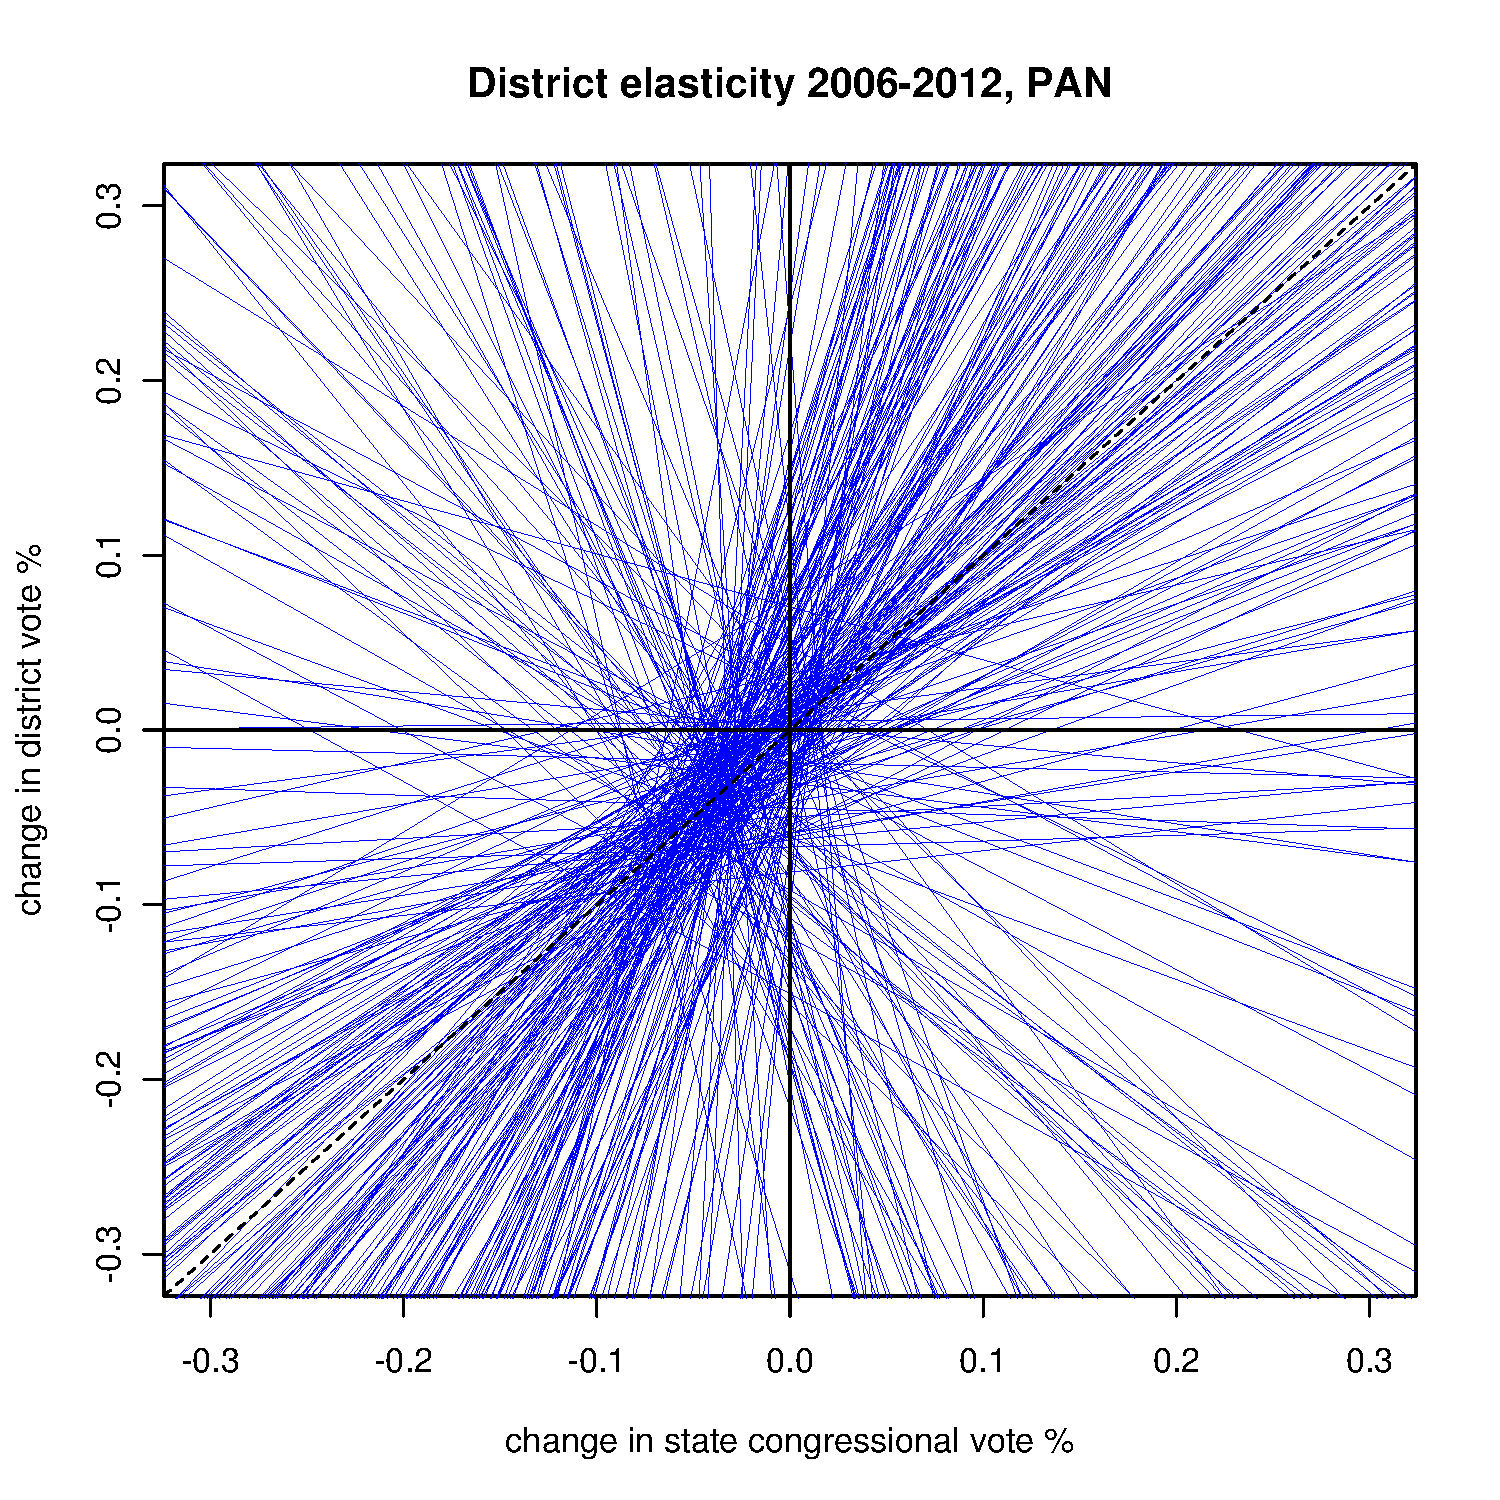
\includegraphics[width=.4\columnwidth]{elastpand0.pdf} & 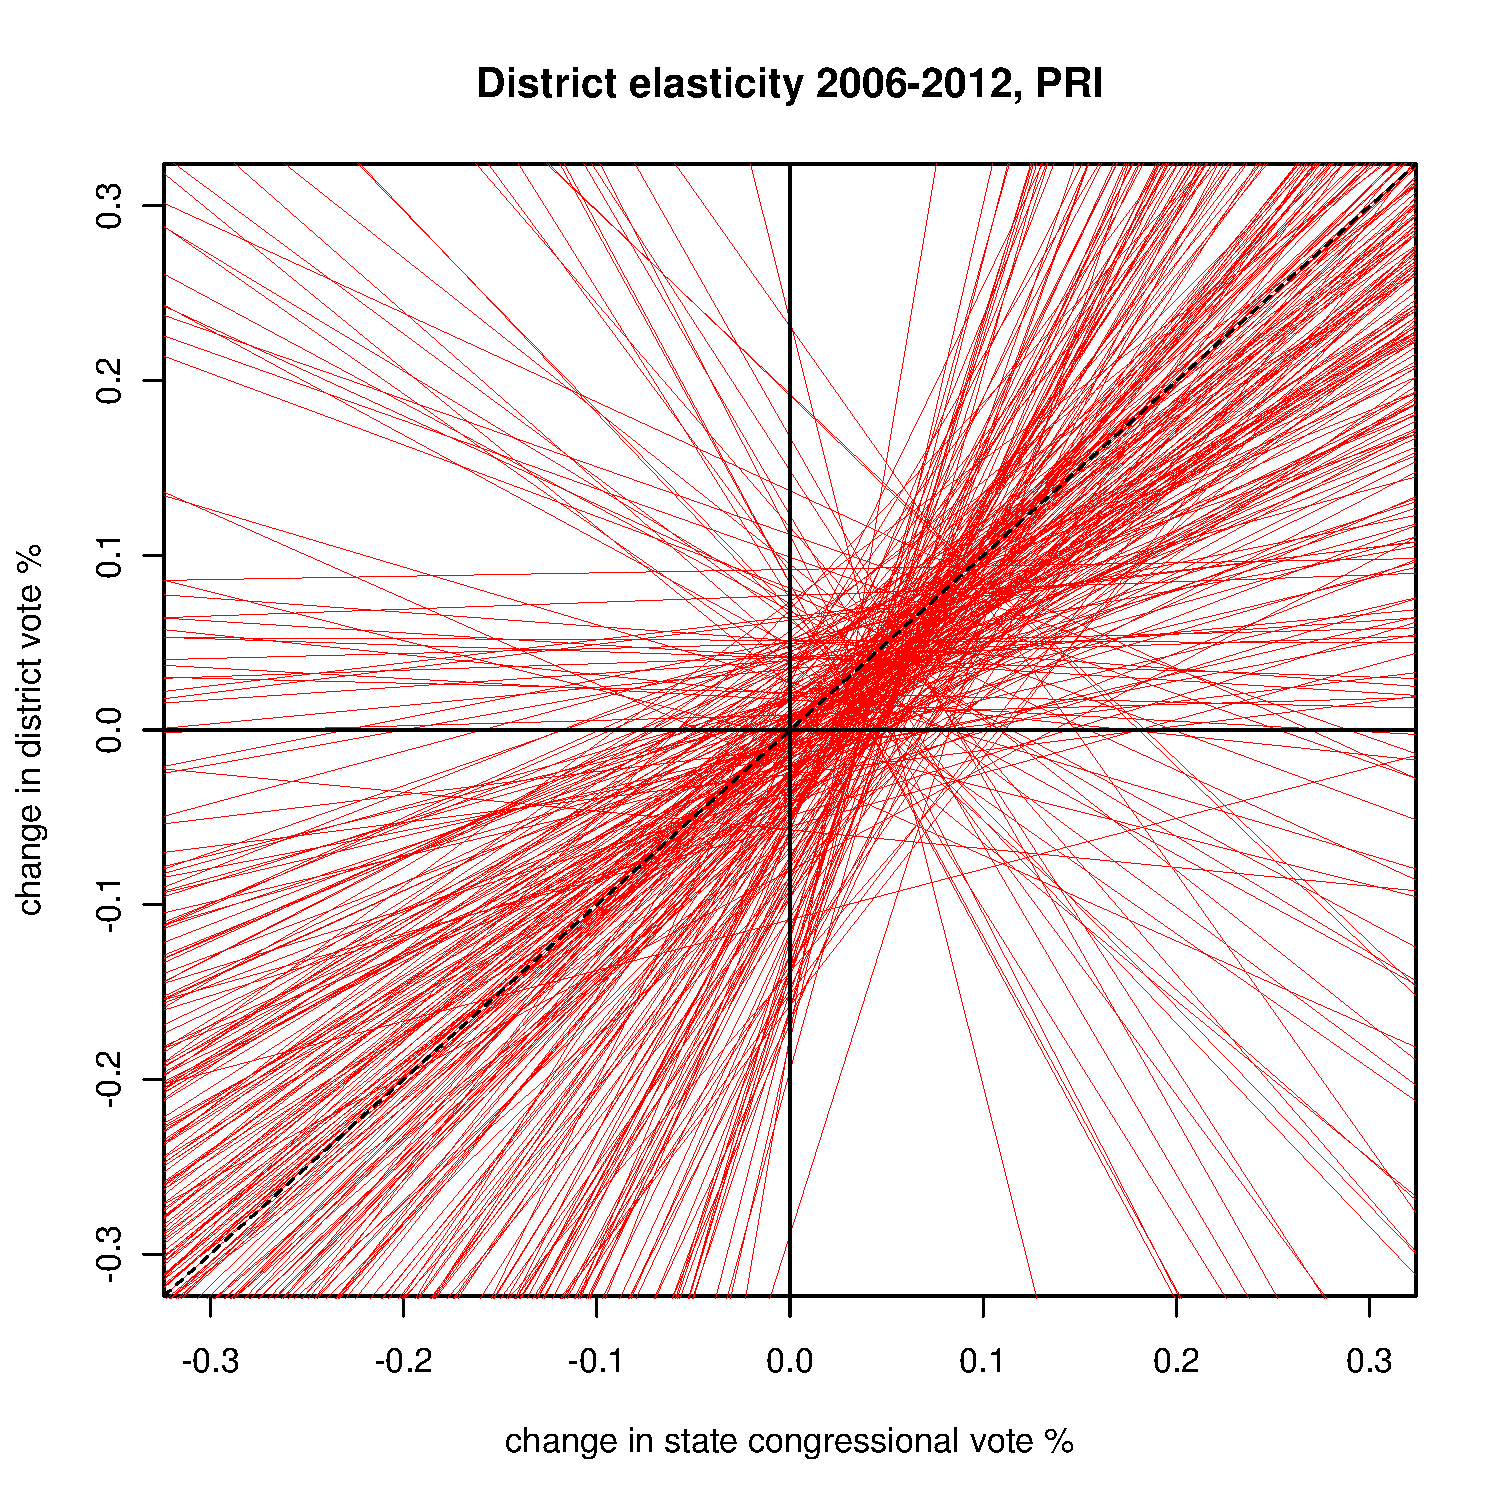
\includegraphics[width=.4\columnwidth]{elastprid0.pdf} \\
    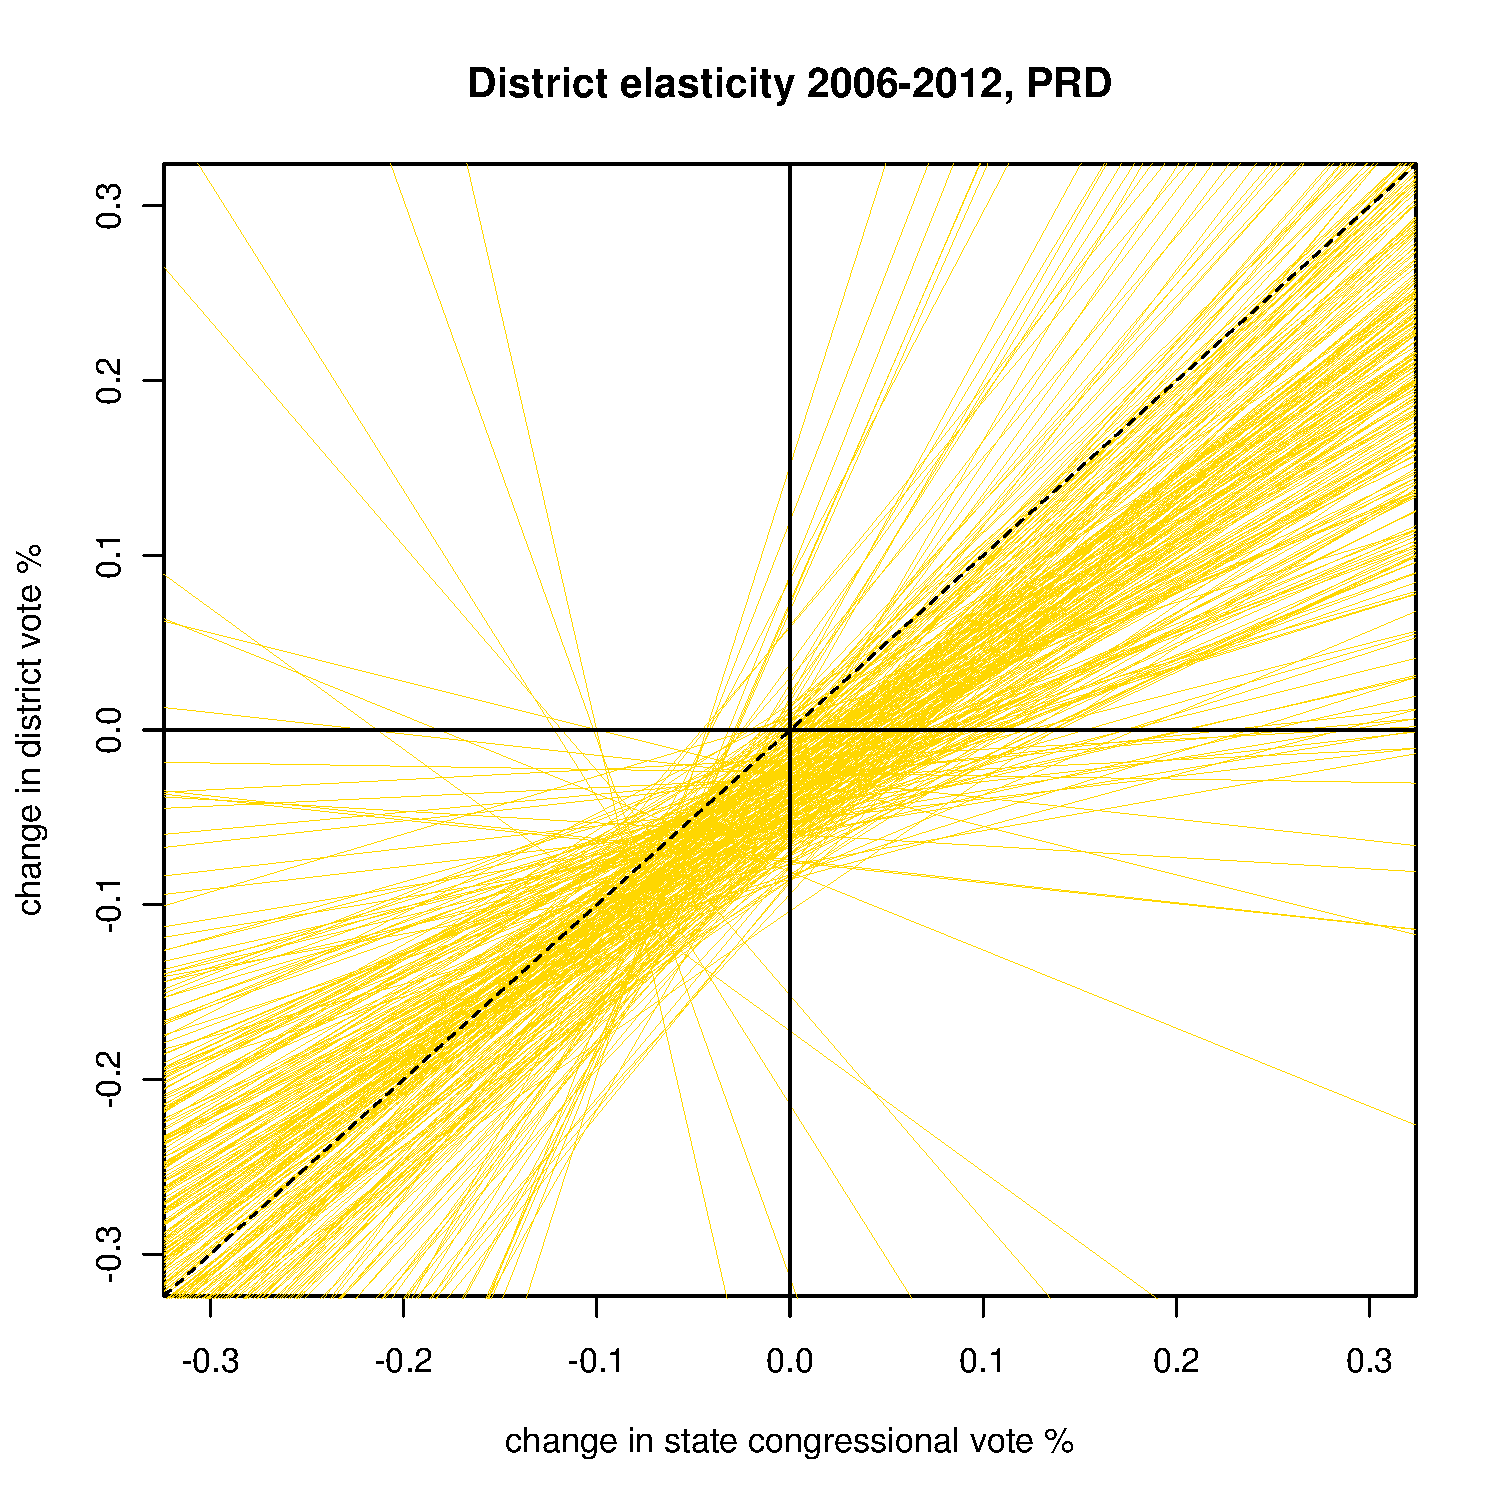
\includegraphics[width=.4\columnwidth]{elastprdd0.pdf} &  \\
  \end{tabular}
  \caption{Parties' district elasticities}\label{F:malmgnat}
\end{center}
\end{figure}



\bibliographystyle{apsr}
%\bibliography{../../../../../mydocs/magar}
\bibliography{../bib/magar}



\end{document}
